\documentclass[border=6pt]{standalone}
\usepackage{tikz}
\usetikzlibrary{arrows.meta,calc,decorations.pathreplacing,positioning}
\begin{document}

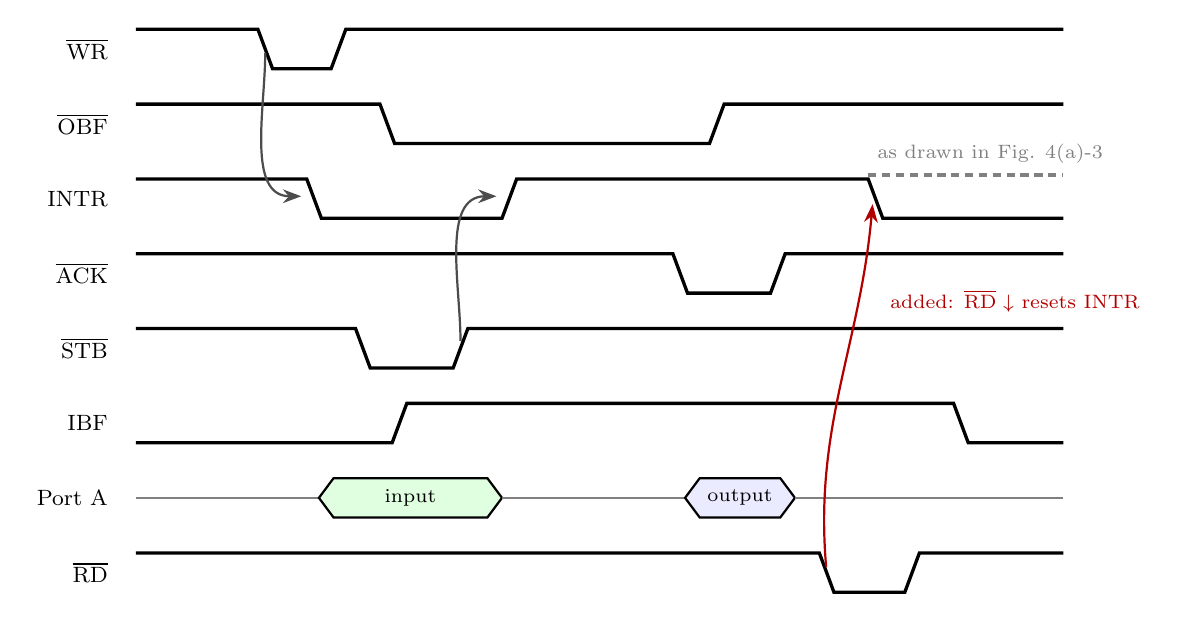
\begin{tikzpicture}[>=Stealth,font=\small,x=1.55cm,y=1cm]
% row 0 y=0
\node[anchor=east,font=\footnotesize,align=right] at (-0.15,0.25) {$\overline{\mathrm{WR}}$};
\draw[very thick] (0,0.5) -- (1,0.5) -- (1.12,0) -- (1.6,0) -- (1.72,0.5) -- (7.6,0.5);
% row 1 y=-0.95
\node[anchor=east,font=\footnotesize,align=right] at (-0.15,-0.7) {$\overline{\mathrm{OBF}}$};
\draw[very thick] (0,-0.45) -- (2,-0.45) -- (2.12,-0.95) -- (4.7,-0.95) -- (4.82,-0.45) -- (7.6,-0.45);
% row 2 y=-1.9
\node[anchor=east,font=\footnotesize,align=right] at (-0.15,-1.65) {INTR};
\draw[very thick] (0,-1.4) -- (1.4,-1.4) -- (1.52,-1.9) -- (3,-1.9) -- (3.12,-1.4) -- (6,-1.4) -- (6.12,-1.9) -- (7.6,-1.9);
% row 3 y=-2.85
\node[anchor=east,font=\footnotesize,align=right] at (-0.15,-2.6) {$\overline{\mathrm{ACK}}$};
\draw[very thick] (0,-2.35) -- (4.4,-2.35) -- (4.52,-2.85) -- (5.2,-2.85) -- (5.32,-2.35) -- (7.6,-2.35);
% row 4 y=-3.8
\node[anchor=east,font=\footnotesize,align=right] at (-0.15,-3.55) {$\overline{\mathrm{STB}}$};
\draw[very thick] (0,-3.3) -- (1.8,-3.3) -- (1.92,-3.8) -- (2.6,-3.8) -- (2.72,-3.3) -- (7.6,-3.3);
% row 5 y=-4.75
\node[anchor=east,font=\footnotesize,align=right] at (-0.15,-4.5) {IBF};
\draw[very thick] (0,-4.75) -- (2.1,-4.75) -- (2.22,-4.25) -- (6.7,-4.25) -- (6.82,-4.75) -- (7.6,-4.75);
% row 6 y=-5.7
\node[anchor=east,font=\footnotesize,align=right] at (-0.15,-5.45) {Port A};
\draw[thick,gray] (0,-5.45) -- (1.5,-5.45);
\draw[thick,fill=green!12] (1.5,-5.45) -- (1.62,-5.2) -- (2.88,-5.2) -- (3,-5.45) -- (2.88,-5.7) -- (1.62,-5.7) -- cycle;
\node[font=\scriptsize] at (2.25,-5.45) {input};
\draw[thick,gray] (3,-5.45) -- (4.5,-5.45);
\draw[thick,fill=blue!8] (4.5,-5.45) -- (4.62,-5.2) -- (5.28,-5.2) -- (5.4,-5.45) -- (5.28,-5.7) -- (4.62,-5.7) -- cycle;
\node[font=\scriptsize] at (4.95,-5.45) {output};
\draw[thick,gray] (5.4,-5.45) -- (7.6,-5.45);
% row 7 y=-6.65
\node[anchor=east,font=\footnotesize,align=right] at (-0.15,-6.4) {$\overline{\mathrm{RD}}$};
\draw[very thick] (0,-6.15) -- (5.6,-6.15) -- (5.72,-6.65) -- (6.3,-6.65) -- (6.42,-6.15) -- (7.6,-6.15);

\draw[->,thick,red!70!black,shorten <=2pt,shorten >=2pt] (5.66,-6.4) to[out=95,in=-95] (6.04,-1.65);
\draw[very thick,gray,densely dashed] (6.0,-1.35) -- (7.6,-1.35);
\node[font=\scriptsize,gray,anchor=south] at (7.0,-1.33) {as drawn in Fig. 4(a)-3};
\node[font=\scriptsize,red!70!black,align=left,anchor=west] at (6.1,-2.95) {added: $\overline{\mathrm{RD}}\downarrow$ resets INTR};
\draw[->,thick,gray!60!black,shorten <=2pt,shorten >=2pt] (1.06,0.27) to[out=-90,in=180] (1.4,-1.62);
\draw[->,thick,gray!60!black,shorten <=2pt,shorten >=2pt] (2.66,-3.53) to[out=90,in=180] (3.0,-1.62);

\end{tikzpicture}
\end{document}
